\subsection{Brienzersee 2014}
\begin{wrapfigure}{r}{0.45\textwidth} 
  \begin{center}
    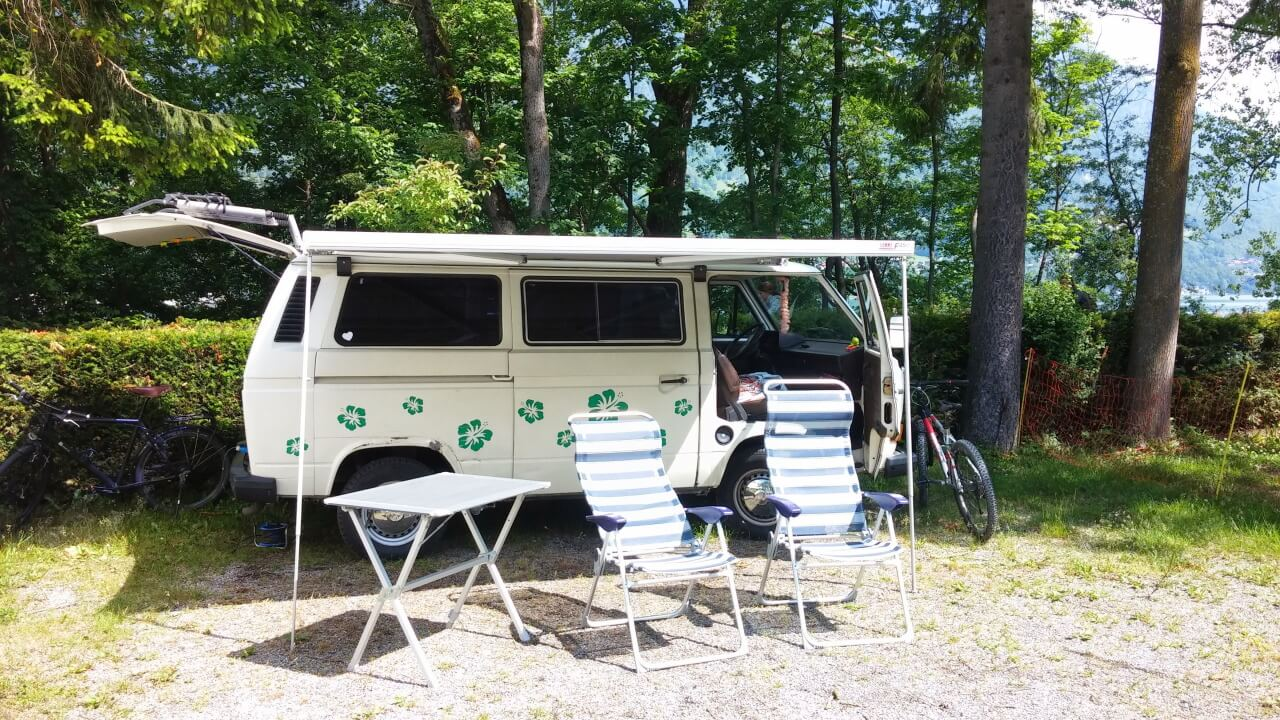
\includegraphics[width=0.4\textwidth]{../Bilder/Brienzersee/1.jpg}
    \caption{Stellplatz in B�nigen}
  \end{center}
\end{wrapfigure} 

Schon fr�h am Morgen, knapp nach Sieben Uhr, machte ich mich daran die letzten Kleider in die Tasche zu werfen.
Fr�hst�ck fiel aus, da auch schon die Velos warteten um auf den Paulchen montiert zu werden.

Kurz nach Neun machten wir uns auf den Weg nachdem uns der Camping Seeg�rtli zusagte und uns Asyl f�r eine Nacht garantieren konnte.
Das Wetter sah eher bescheiden aus, nichtsdestotrotz machten wir uns guten Mutes auf den Weg.
In die falsche Richtung.
Macht der Gewohnheit wollte ich Richtung Z�rich auf die Autobahn.
Meine Navigatorin hatte keine Einw�nde und zeigte sich eher �berrascht als ich ihr kurz nach der Einfahrt meinen Lapsus kundtat.
Nach einem weiteren kurzen Abstecher in Luzern (Macht der Gewohnheit zum zweiten, wenn man von Z�rich kommt, Ausfahrt Luzern nehmen.)
waren wir schlussendlich auf dem Weg �ber den Br�nig.
Das Wetter verbesserte sich schlagartig nach dem wir den Pass �berquert hatten und die Wolken gaben den Blick Richtung Tal frei.
Nach der geeigneten Stellplatz suche ging es Nahtlos weiter mit der Suche nach einem Restaurant.
Gefunden und schnell die Pl�ne f�r den weiteren Nachmittag geschmiedet.
Neben der Reception sind wir noch dem Internet �ber den Weg gelaufen.
Nie gedacht, dass das Internet so aussieht.
Ist halt Neuland f�r uns alle.
N�chste Aktion: Die Reichenbachf�lle sollten begutachtet werden.
Das Ganze mit einer kurzen Wanderung eingerahmt von Schifffahrten.
Mit dem Schiff ging es nach Iseltwald, per pedes bis zum Grand Hotel Giessbach.
Alles immer am Ufer des sch�nen Brienzersee entlang.
Nach dem Besuch der beeindruckenden Wassermassen ging es ein weiteres Mal gem�tlich mit dem Schiff zur�ck nach B�nigen.
Der Abdruck der sich in der Nasengegend langsam abzeichnete zeigte an, dass ein gewisses Wettergl�ck bestand.

\begin{figure}[H]
   \centering
      %\subfloat[CAPTION]{BILDERCODE}\qquad
   \subfloat{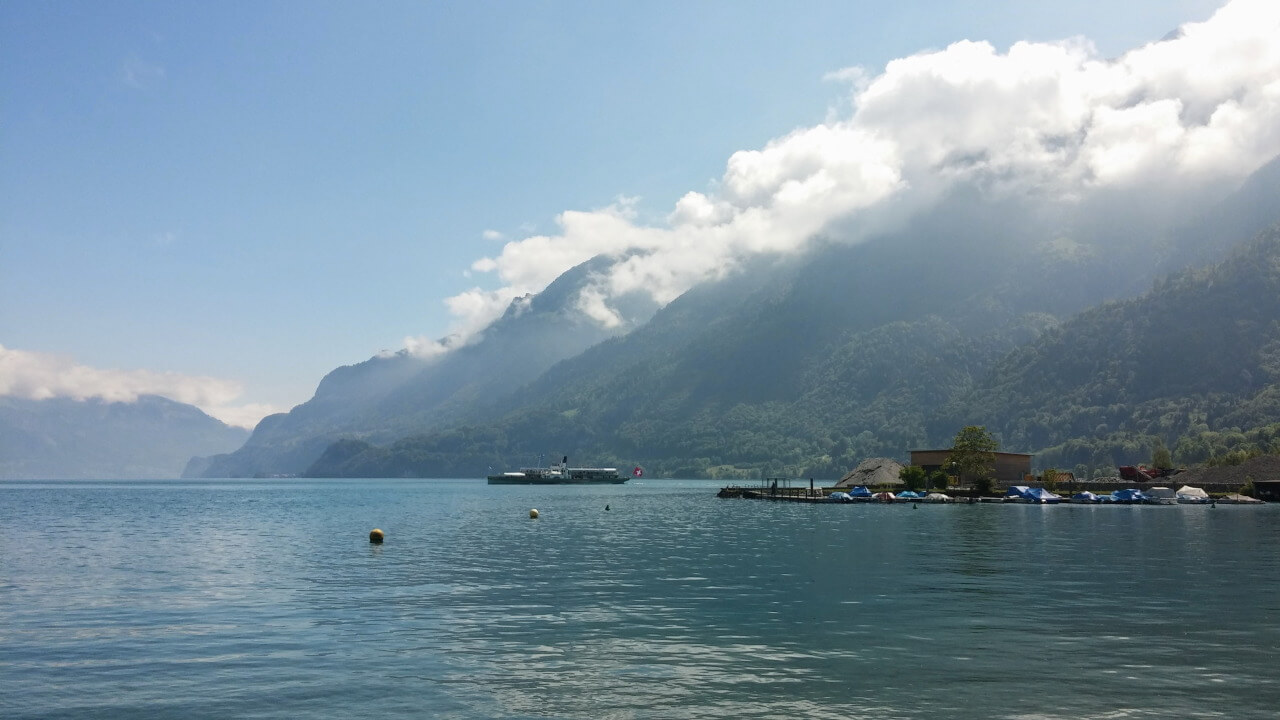
\includegraphics [width=0.3\textwidth]{../Bilder/Brienzersee/2.jpg}}\quad
   \subfloat{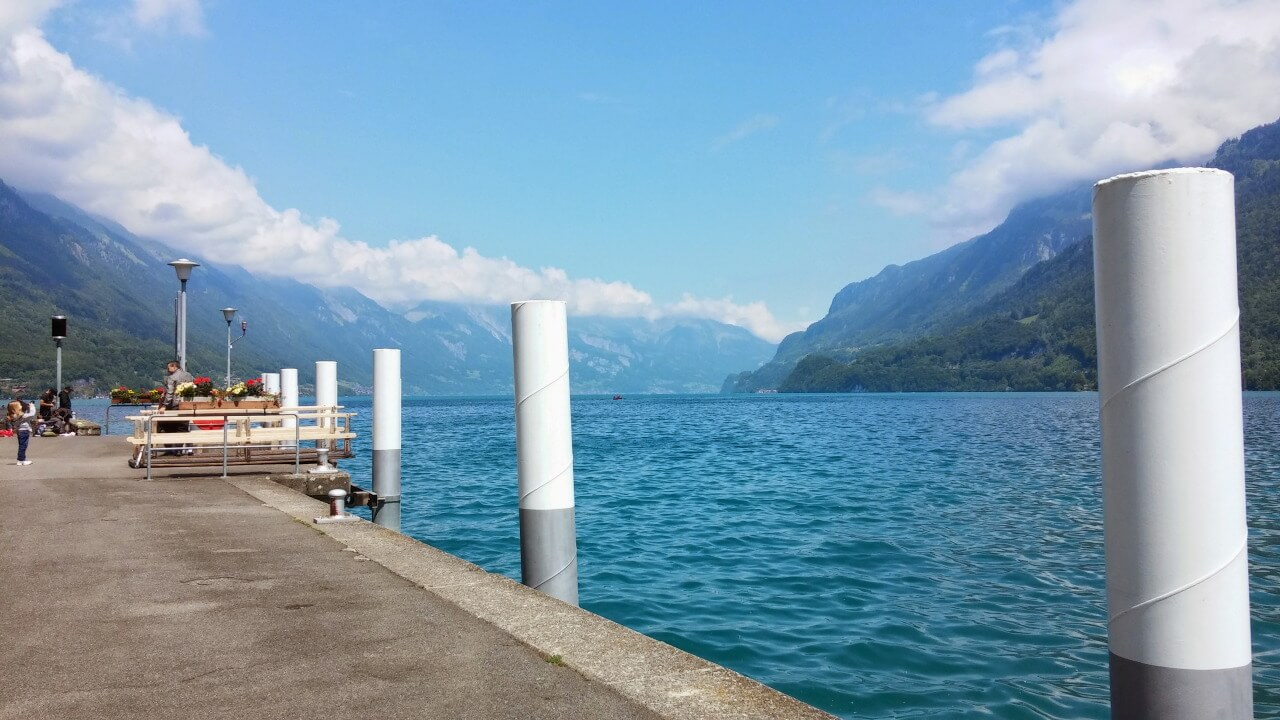
\includegraphics [width=0.3\textwidth]{../Bilder/Brienzersee/5.jpg}}\quad
   \subfloat{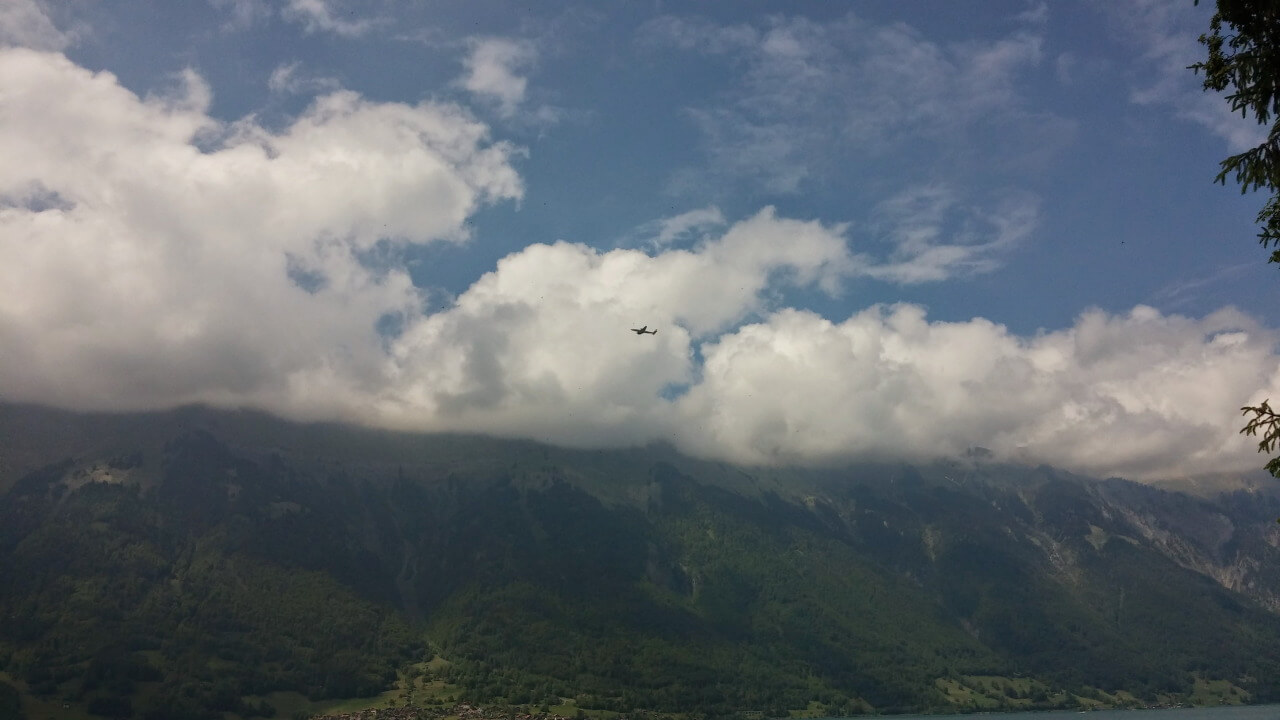
\includegraphics [width=0.3\textwidth]{../Bilder/Brienzersee/6.jpg}}\quad
   \caption[Brienzersee]{Brienzersee}
\end{figure}

Sobald sich jedoch die Sonne aus dem Staub machte war es vorbei mit den angenehmen Temperaturen.
Der kurze Spaziergang zur Pizzeria musste schon mit erheblich mehr Kleidung angetreten werden.
Chantal zeigte erste Anzeichen von �berheblichen Sonnenkonsum und so zogen wir uns nach dem Nachtessen zur�ck um einen Film im Bussli zu geniessen.

Nach einer k�hlen aber langen Nacht, war nicht mehr viel mit herumlungern.
Es war schon nach 10 Uhr.
Die Gipfeli im Campingcafe gingen zu neige und wir sicherten uns gerade die letzten.
Es gab noch dies und das in den Bus zu packen und dann hiess es Abschied nehmen von Pipo und seinem sympathischen Herrchen und Frauchen.
Thun war leicht zu finden und wir besuchten kurz den Schlossberg.
Die ganze Stadt war auf den Beinen und die sch�nen Restaurants und Cafes brummten regelrecht.
Wir genossen ein Zmittag an der Sonne und beschlossen direkt �ber Bern Richtung Baden zu fahren.
Das Gep�ck in den Twingo umzuladen und so den Bus in Nussbaumen zu parkieren.
Schon auf dem Weg zur Autobahn Richtung Bern ist uns ein kleiner Hacken in unserem wunderbaren Plan aufgefallen.
Die beiden Fahrr�der die uns auf dem Paulchen begleiteten passten garantiert nicht in den Twingo.
Alles kehrt und so kamen wir dazu noch einmal den Br�nig zu befahren, dieses Mal bei sch�nstem Wetter.
Gl�cklich und mit roter Nase kamen wir am Sonntag Abend wieder in Luzern an.

\begin{figure}[H]
    \centering
    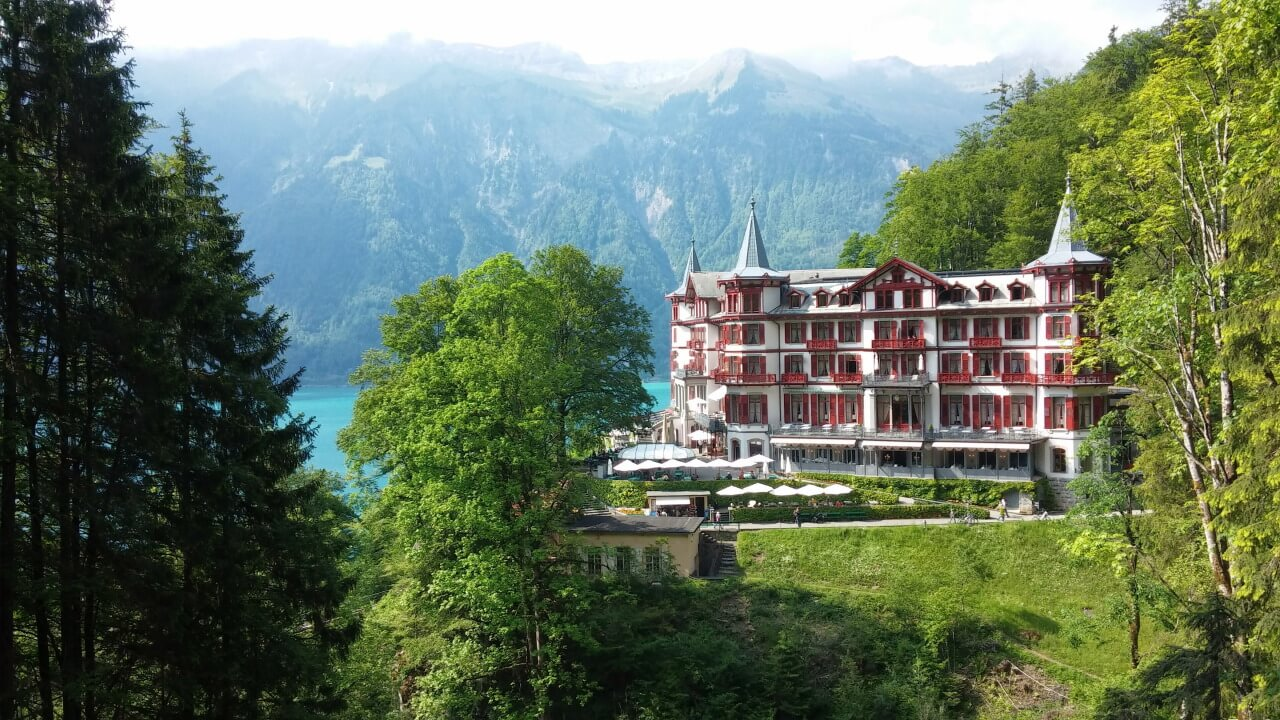
\includegraphics[width=0.5\textwidth]{../Bilder/Brienzersee/14.jpg}
    \caption{Giessbachf�lle}
    \label{img:Brienzersee}
\end{figure}

\begin{figure}[H]
    \centering
    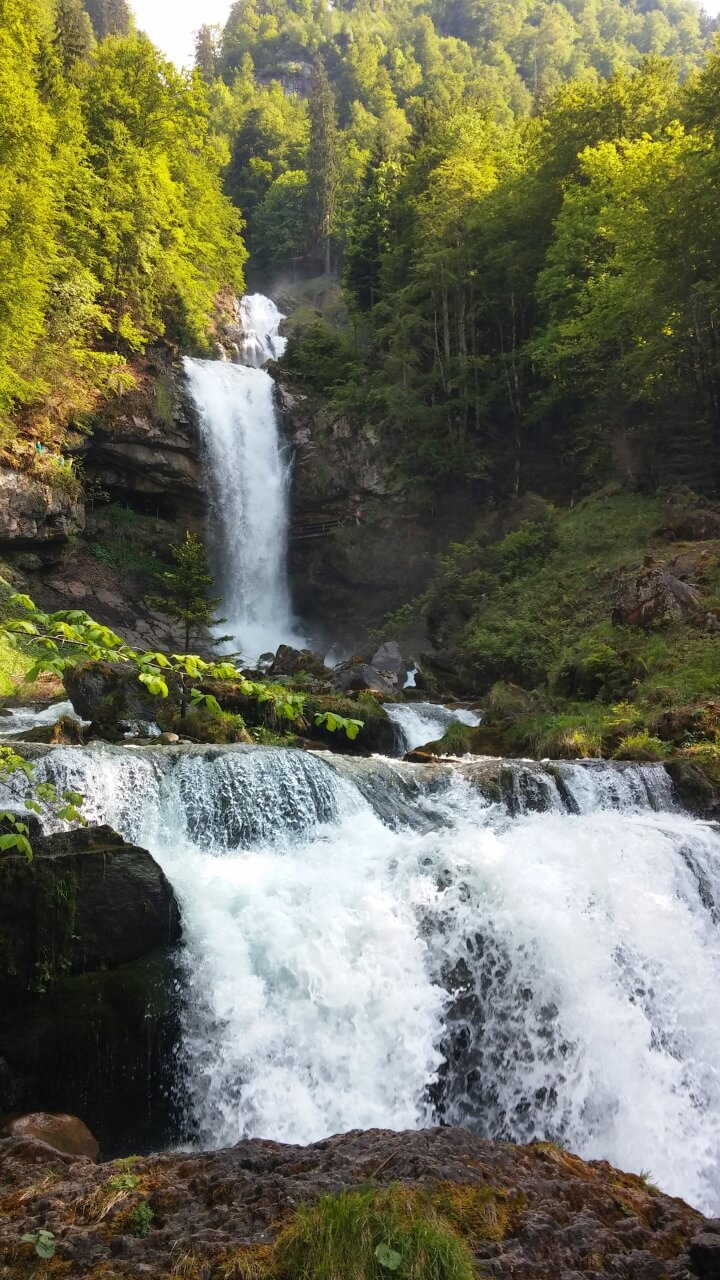
\includegraphics[width=0.4\textwidth]{../Bilder/Brienzersee/12.jpg}
    \caption{Giessbachf�lle}
    \label{img:Brienzersee2}
\end{figure}
